% Chapter 3: Probability and Information Theory

\chapter{Probability and Information Theory}
\label{chap:probability}

This chapter introduces fundamental concepts from probability theory and information theory that are essential for understanding machine learning and deep learning. Topics include probability distributions, conditional probability, expectation, variance, entropy, and mutual information.

\begin{learningobjectives}
\objective{Probability foundations and grasp the intuitive meaning of probability distributions, both discrete and continuous, and how they model uncertainty in real-world scenarios}
\objective{Conditional probability and use Bayes' theorem to update beliefs with new evidence and understand its central role in machine learning algorithms}
\objective{Statistical measures and compute expectation, variance, and covariance to characterize the behavior of random variables and their relationships}
\objective{Common distributions and recognize when to use Bernoulli, Gaussian, and other probability distributions in machine learning contexts}
\objective{Information content and use entropy, cross-entropy, and KL divergence to measure uncertainty and information in data and models}
\objective{Information theory and connect information-theoretic concepts to loss functions, model selection, and representation learning in deep neural networks}
\end{learningobjectives}

% Chapter 3, Section 1: Probability Distributions

\section{Probability Distributions \difficultyInline{beginner}}
\label{sec:probability-distributions}

Probability distributions are mathematical functions that describe how probabilities are distributed across different possible outcomes of a random variable, providing the fundamental framework for modeling uncertainty in data and making predictions in machine learning and deep learning applications.

\subsection{Intuition: What is Probability?}

Imagine you're playing a game of dice where you roll a standard six-sided die with numbers 1 through 6. Before rolling, you know that each face has an equal chance of appearing, meaning that if you roll the die many times, each number will appear approximately one-sixth of the time. This "chance" is what we call probability - a number between 0 and 1 that quantifies how likely an event is to occur, where 0 means impossible and 1 means certain. In machine learning, we face uncertainty everywhere, from data uncertainty about whether the next customer will click on an ad, to model uncertainty about how confident our neural network is in its prediction, to parameter uncertainty about what the best value is for our model's weights. Probability distributions are mathematical tools that help us model and work with this uncertainty systematically, providing a rigorous framework for making decisions under uncertainty and quantifying the confidence we can have in our predictions and model parameters.

\subsection{Visualizing Probability}

Consider a simple example: predicting whether it will rain tomorrow. We might say there's a 30\% chance of rain, which means that if we could repeat tomorrow 100 times, rain would occur about 30 times, the probability of rain is 0.3, and the probability of no rain is 0.7. This intuitive understanding of probability helps us visualize how probability distributions work - they assign numerical values to different outcomes, showing us not just what can happen, but how likely each outcome is to occur.

\begin{figure}[h]
\centering
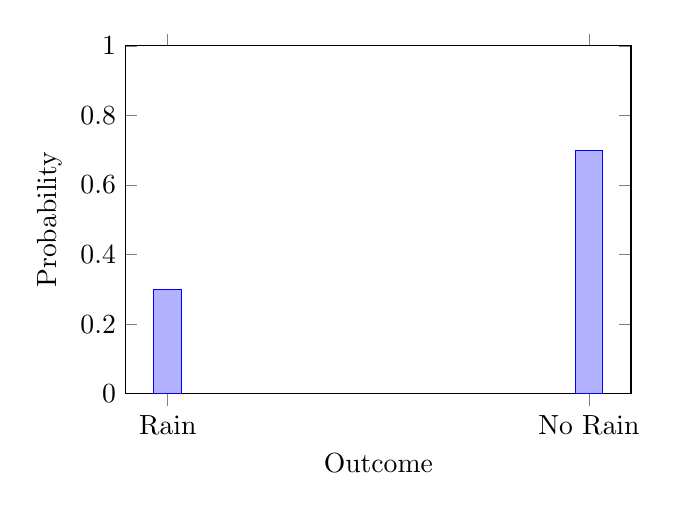
\begin{tikzpicture}
\begin{axis}[
    ybar,
    ylabel={Probability},
    xlabel={Outcome},
    xtick={1,2},
    xticklabels={Rain, No Rain},
    ymin=0,
    ymax=1,
    width=8cm,
    height=6cm
]
\addplot coordinates {(1,0.3) (2,0.7)};
\end{axis}
\end{tikzpicture}
\caption{Probability distribution for rain prediction}
\label{fig:rain-probability}
\end{figure}

Probability theory provides a mathematical framework for quantifying uncertainty. In deep learning, we use probability distributions to model uncertainty in data, model parameters, and predictions.

\subsection{Discrete Probability Distributions}

Discrete probability distributions deal with outcomes that can be counted and listed explicitly, such as coin flips with heads or tails, dice rolls with numbers 1 through 6, or email classification with spam or not spam. These distributions assign probabilities to each possible outcome, where the sum of all probabilities equals 1, representing the fact that one of the possible outcomes must occur.

A discrete random variable $X$ takes values from a countable set. The \textbf{probability mass function} (PMF) $P(X=x)$ assigns probabilities to each possible value:

\begin{equation}
P(X=x) \geq 0 \quad \text{for all } x
\end{equation}

\begin{equation}
\sum_{x} P(X=x) = 1
\end{equation}

\subsubsection{Example: Fair Coin}

For a fair coin, we have:
\begin{align}
P(X=0) &= 0.5 \quad \text{(Tails)} \\
P(X=1) &= 0.5 \quad \text{(Heads)}
\end{align}

\begin{figure}[h]
\centering
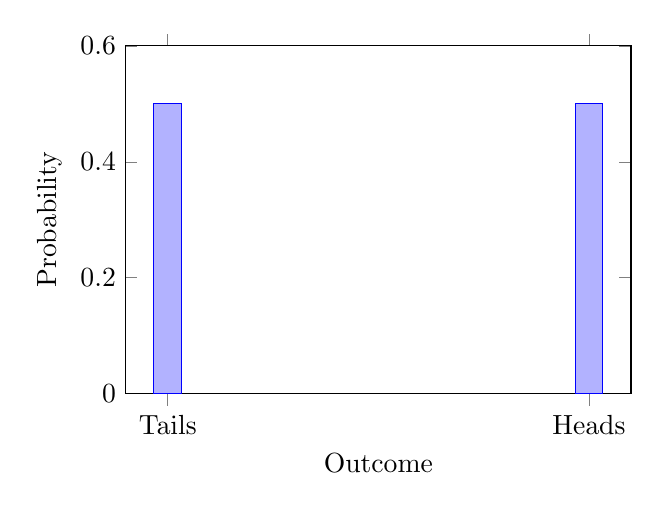
\begin{tikzpicture}
\begin{axis}[
    ybar,
    ylabel={Probability},
    xlabel={Outcome},
    xtick={0,1},
    xticklabels={Tails, Heads},
    ymin=0,
    ymax=0.6,
    width=8cm,
    height=6cm
]
\addplot coordinates {(0,0.5) (1,0.5)};
\end{axis}
\end{tikzpicture}
\caption{Probability mass function for a fair coin}
\label{fig:coin-pmf}
\end{figure}

\subsection{Continuous Probability Distributions}

Continuous probability distributions deal with variables that can take any value within a continuous range, such as the height of people which can be 170 cm, 170.5 cm, 170.52 cm, and so on, or temperature which can be 22.3°C, 22.34°C, 22.341°C, and so on, or neural network weights which can be 0.1234, 0.12345, 0.123456, and so on. Since there are infinitely many possible values, we can't assign probabilities to individual points, but instead use density functions that describe how "concentrated" the probability is in different regions of the continuous space.

A continuous random variable can take any value in a continuous range. We describe it using a \textbf{probability density function} (PDF) $p(x)$:

\begin{equation}
p(x) \geq 0 \quad \text{for all } x
\end{equation}

\begin{equation}
\int_{-\infty}^{\infty} p(x) \, dx = 1
\end{equation}

The probability that $X$ falls in an interval $[a, b]$ is:

\begin{equation}
P(a \leq X \leq b) = \int_a^b p(x) \, dx
\end{equation}

\begin{examplebox}{Normal Distribution}
The most common continuous distribution is the \textbf{normal (Gaussian) distribution}, which looks like a bell curve:

\begin{center}
\begin{tikzpicture}
\begin{axis}[
    ylabel={Probability Density},
    xlabel={Value},
    domain=-3:3,
    width=10cm,
    height=6cm,
    samples=100,
    grid=major,
    grid style={line width=.1pt, draw=gray!10},
    major grid style={line width=.2pt, draw=gray!50}
]
\addplot[bookpurple, thick] {1/sqrt(2*pi) * exp(-x^2/2)};
\addplot[bookred, thick] {1/sqrt(2*pi*0.5) * exp(-(x-0.5)^2/(2*0.5))};
\end{axis}
\end{tikzpicture}
\end{center}

The area under the curve between any two points gives the probability of the variable falling in that range.

\begin{center}
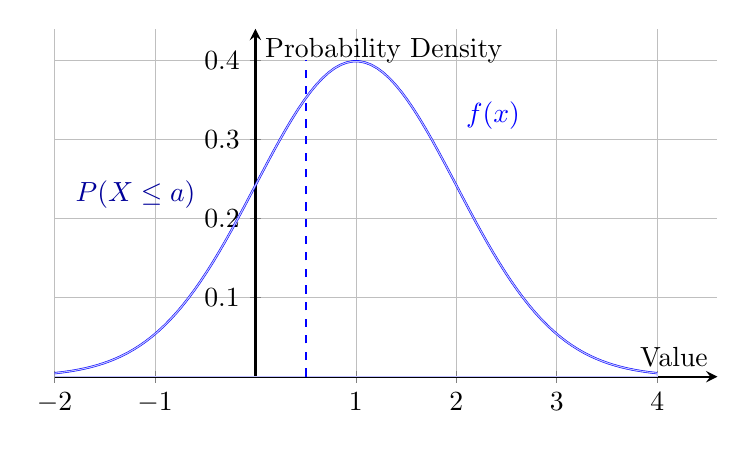
\begin{tikzpicture}
\begin{axis}[
    ylabel={Probability Density},
    xlabel={Value},
    domain=-2:4,
    width=10cm,
    height=6cm,
    samples=100,
    grid=major,
    grid style={line width=.1pt, draw=gray!10},
    major grid style={line width=.2pt, draw=gray!50},
    axis lines=middle,
    axis line style=thick,
    enlargelimits=upper
]
% Normal distribution
\addplot[blue,thick] {1/sqrt(2*pi) * exp(-(x-1)^2/2)};
% Fill area under curve from -2 to 0.5
\addplot[blue!25, fill opacity=0.3] {1/sqrt(2*pi) * exp(-(x-1)^2/2)} \closedcycle;
% Vertical line at a=0.5
\addplot[blue,dashed,thick] coordinates {(0.5,0) (0.5,0.4)};
\node[blue,below] at (axis cs:0.5,0) {$a$};
\node[blue,above right] at (axis cs:2,0.3) {$f(x)$};
\node[blue!60!black,above left] at (axis cs:-0.5,0.2) {$P(X\leq a)$};
\end{axis}
\end{tikzpicture}
\end{center}
\end{examplebox}

\subsection{Joint and Marginal Distributions}

In real-world scenarios, we often deal with multiple variables simultaneously, such as weather prediction involving both temperature and humidity, image classification involving pixel values at different positions, or stock prices involving multiple stocks in a portfolio. The joint distribution tells us about the probability of combinations of values across all variables, while marginal distributions tell us about individual variables when we ignore the others, providing a way to understand both the relationships between variables and the behavior of individual variables in isolation.

\begin{examplebox}{Weather Data}
Consider a simple weather dataset with two variables:
\begin{itemize}
    \item $X$: Temperature (Hot/Cold)
    \item $Y$: Humidity (High/Low)
\end{itemize}

\begin{center}
\begin{tabular}{|c|c|c|c|}
\hline
 & $Y=$ High & $Y=$ Low & \textbf{Marginal} \\
\hline
$X=$ Hot & 0.3 & 0.2 & \textbf{0.5} \\
$X=$ Cold & 0.1 & 0.4 & \textbf{0.5} \\
\hline
\textbf{Marginal} & \textbf{0.4} & \textbf{0.6} & \textbf{1.0} \\
\hline
\end{tabular}
\end{center}

For multiple random variables $X$ and $Y$, the \textbf{joint distribution} $P(X, Y)$ describes their combined behavior. The \textbf{marginal distribution} is obtained by summing (or integrating) over the other variable:

\begin{equation}
P(X=x) = \sum_{y} P(X=x, Y=y)
\end{equation}

For continuous variables:

\begin{equation}
p(x) = \int p(x, y) \, dy
\end{equation}

From our weather example:
\begin{itemize}
    \item $P(X=\text{Hot}) = 0.3 + 0.2 = 0.5$ (marginal probability of hot weather)
    \item $P(Y=\text{High}) = 0.3 + 0.1 = 0.4$ (marginal probability of high humidity)
\end{itemize}
\end{examplebox}

% Chapter 3, Section 2: Conditional Probability and Bayes' Rule

\section{Conditional Probability and Bayes' Rule \difficultyInline{beginner}}
\label{sec:conditional-probability}

This section introduces the fundamental concepts of conditional probability and Bayes' theorem, which are essential for understanding how to update beliefs with new information in machine learning.

\subsection{Intuition: Updating Beliefs with New Information}

Imagine you're a doctor trying to diagnose a patient. Initially, you might think there's a 5\% chance the patient has a rare disease. But then the patient tells you they have a specific symptom that's present in 80\% of people with that disease. How should you update your belief?

This is exactly what \textbf{conditional probability} helps us do - it tells us how to update our beliefs when we get new information.

\subsection{Conditional Probability}

\begin{definition}[Conditional Probability]
The conditional probability of $X$ given $Y$ is defined as:
\begin{equation}
P(X|Y) = \frac{P(X, Y)}{P(Y)}
\end{equation}
This quantifies how the probability of $X$ changes when we know the value of $Y$. This concept is fundamental to understanding how new information updates our beliefs about uncertain events, allowing us to make more informed decisions based on the evidence we observe.
\end{definition}

\begin{examplebox}{Medical Diagnosis}
Let's make this concrete with our medical example:
\begin{itemize}
    \item $D$: Patient has the disease (1 = yes, 0 = no)
    \item $S$: Patient has the symptom (1 = yes, 0 = no)
\end{itemize}

From medical records, we know:
\begin{itemize}
    \item $P(D=1) = 0.05$ (5\% of population has the disease)
    \item $P(S=1|D=1) = 0.8$ (80\% of diseased patients have the symptom)
    \item $P(S=1|D=0) = 0.1$ (10\% of healthy patients have the symptom)
\end{itemize}

If a patient has the symptom, what's the probability they have the disease?

Using Bayes' theorem (which we'll derive next):
\begin{align}
P(D=1|S=1) &= \frac{P(S=1|D=1)P(D=1)}{P(S=1)} \\
&= \frac{0.8 \times 0.05}{0.8 \times 0.05 + 0.1 \times 0.95} \\
&= \frac{0.04}{0.04 + 0.095} \\
&= \frac{0.04}{0.135} \approx 0.296
\end{align}

So even with the symptom, there's only about a 30\% chance the patient has the disease!
\end{examplebox}

\subsection{Independence}

Two events are independent if knowing one doesn't change our belief about the other, such as rolling two dice where the result of the first die doesn't affect the second, or they can be dependent like weather and clothing choice where knowing it's raining affects the probability you'll wear a raincoat. Two random variables $X$ and $Y$ are independent if $P(X, Y) = P(X)P(Y)$, which means that the joint probability equals the product of the individual probabilities, or equivalently, $P(X|Y) = P(X)$ and $P(Y|X) = P(Y)$, indicating that knowing the value of one variable doesn't change our belief about the other.

\begin{examplebox}{Independent vs Dependent Variables}
Consider two scenarios:

\textbf{Scenario 1 (Independent):} Flipping two coins
\begin{itemize}
    \item $P(\text{First coin = Heads}) = 0.5$
    \item $P(\text{Second coin = Heads}) = 0.5$
    \item $P(\text{Both Heads}) = 0.5 \times 0.5 = 0.25$ \checkmark
\end{itemize}

\textbf{Scenario 2 (Dependent):} Drawing cards without replacement
\begin{itemize}
    \item $P(\text{First card = Ace}) = 4/52 = 1/13$
    \item $P(\text{Second card = Ace}) = 3/51$ (if first was Ace) or $4/51$ (if first wasn't Ace)
    \item The probability of the second card depends on what the first card was
\end{itemize}
\end{examplebox}

\subsection{Bayes' Theorem}

\subsubsection{Intuition: The Most Important Formula in Machine Learning}

Bayes' theorem is like a "belief update machine." It tells us how to revise our initial beliefs (prior) when we observe new evidence, to get our updated beliefs (posterior).

\begin{theorem}[Bayes' Theorem]
Bayes' theorem is fundamental to probabilistic inference:

\begin{equation}
P(X|Y) = \frac{P(Y|X)P(X)}{P(Y)}
\end{equation}
\end{theorem}

\subsubsection{Understanding Each Component}

In machine learning terminology:
\begin{itemize}
    \item $P(X)$ is the \textbf{prior} probability - what we believed before seeing the data
    \item $P(Y|X)$ is the \textbf{likelihood} - how likely the data is given our hypothesis
    \item $P(X|Y)$ is the \textbf{posterior} probability - what we believe after seeing the data
    \item $P(Y)$ is the \textbf{evidence} or marginal likelihood - the probability of observing the data
\end{itemize}

The formula can be read as: "Posterior = (Likelihood × Prior) ÷ Evidence"

\subsection{Application to Machine Learning}

Bayes' theorem forms the basis of several important machine learning techniques. Bayesian inference provides a framework for updating beliefs about model parameters as new data becomes available, allowing for principled uncertainty quantification and decision-making under uncertainty. Naive Bayes classifiers use the assumption of feature independence to efficiently compute posterior probabilities for classification tasks, making them particularly useful for text classification and spam detection applications. Maximum a posteriori (MAP) estimation combines prior knowledge about parameters with observed data to find the most likely parameter values, providing a principled way to incorporate domain expertise into machine learning models. Bayesian neural networks extend traditional neural networks by treating weights as random variables with probability distributions, enabling uncertainty quantification in predictions and providing more robust estimates of model confidence.

Given data $\mathcal{D}$ and model parameters $\theta$:

\begin{equation}
P(\theta|\mathcal{D}) = \frac{P(\mathcal{D}|\theta)P(\theta)}{P(\mathcal{D})}
\end{equation}

% Chapter 3, Section 3: Expectation, Variance, and Covariance

\section{Expectation, Variance, and Covariance \difficultyInline{beginner}}
\label{sec:expectation-variance}

Expectation, variance, and covariance are fundamental statistical measures that characterize the behavior of random variables, providing essential tools for understanding data distributions, relationships between variables, and uncertainty quantification in machine learning and deep learning applications.

\subsection{Intuition: Characterizing Random Variables}

When we have a random variable, we often want to summarize its behavior with a few key numbers that capture the essential characteristics of the distribution. The expected value or mean represents the "center" or "typical" value around which the data is distributed, while variance measures how much the values spread out from the center, indicating the degree of uncertainty or variability in the data. Covariance tells us how two variables move together, revealing whether they tend to increase or decrease simultaneously, which is crucial for understanding relationships between different features or measurements. Think of it like describing a person: the mean height represents the average height of people in a group, the variance in height shows how much heights vary between tall and short people, and the covariance of height and weight reveals whether taller people tend to weigh more, providing insights into the relationships between different characteristics.

\subsection{Expectation}

The \textbf{expected value} or \textbf{mean} of a function $f(x)$ with respect to distribution $P(x)$ is:

For discrete variables:
\begin{equation}
\mathbb{E}_{x \sim P}[f(x)] = \sum_{x} P(x) f(x)
\end{equation}

For continuous variables:
\begin{equation}
\mathbb{E}_{x \sim p}[f(x)] = \int p(x) f(x) \, dx
\end{equation}

\begin{remark}
Discrete expectation is a special case of continuous expectation. When we have a discrete distribution with probability mass function $P(x)$, we can think of it as a continuous distribution using Dirac delta functions: $p(x) = \sum_i P(x_i) \delta(x - x_i)$. The integral $\int p(x) f(x) \, dx$ then becomes $\sum_i P(x_i) f(x_i)$, which is exactly the discrete expectation formula. This unified view helps us understand that both discrete and continuous expectations follow the same fundamental principle of weighted averaging.
\end{remark}

\begin{examplebox}{Expected Value of Dice}
For a fair six-sided die:
\begin{align}
\mathbb{E}[X] &= \sum_{x=1}^{6} x \cdot P(X=x) \\
&= 1 \cdot \frac{1}{6} + 2 \cdot \frac{1}{6} + \cdots + 6 \cdot \frac{1}{6} \\
&= \frac{1+2+3+4+5+6}{6} = \frac{21}{6} = 3.5
\end{align}

The expected value is 3.5, even though we can never actually roll 3.5!

\begin{center}
\begin{tikzpicture}
\begin{axis}[
    ybar,
    ylabel={Probability},
    xlabel={Dice Value},
    xtick={1,2,3,4,5,6},
    ymin=0,
    ymax=0.2,
    width=10cm,
    height=6cm
]
\addplot coordinates {(1,1/6) (2,1/6) (3,1/6) (4,1/6) (5,1/6) (6,1/6)};
\draw[bookred, thick] (axis cs:3.5,0) -- (axis cs:3.5,0.2);
\node[bookred] at (axis cs:3.5,0.18) {$\mathbb{E}[X] = 3.5$};
\end{axis}
\end{tikzpicture}
\end{center}
\end{examplebox}

\subsection{Variance}

\subsubsection{Intuition: Measuring Spread}

Variance tells us how "spread out" the values are around the mean. Imagine two dart players with very different playing styles. The first player has low variance in their throws - every dart lands very close to the bullseye, creating a tight cluster of holes around the center. This player is consistent and precise, with their throws showing little variation from the target. The second player has high variance in their throws - their darts are scattered all over the board, some landing far to the left, others to the right, some high, some low. This player is inconsistent and unpredictable, with their throws showing large variation from the target. Variance quantifies this difference in consistency, measuring how much the individual values deviate from the average or expected value.

The \textbf{variance} measures the spread of a distribution:

\begin{equation}
\text{Var}(X) = \mathbb{E}[(X - \mathbb{E}[X])^2] = \mathbb{E}[X^2] - (\mathbb{E}[X])^2
\end{equation}

The \textbf{standard deviation} is $\sigma = \sqrt{\text{Var}(X)}$.

\subsubsection{Example: Variance of Dice}

For our fair die:
\begin{align}
\text{Var}(X) &= \mathbb{E}[X^2] - (\mathbb{E}[X])^2 \\
&= \left(\frac{1^2 + 2^2 + \cdots + 6^2}{6}\right) - (3.5)^2 \\
&= \frac{91}{6} - 12.25 = 15.17 - 12.25 = 2.92
\end{align}

So $\sigma = \sqrt{2.92} \approx 1.71$.

\begin{center}
\begin{tikzpicture}
\begin{axis}[
    ybar,
    ylabel={Probability},
    xlabel={Dice Value},
    xtick={1,2,3,4,5,6},
    ymin=0,
    ymax=0.2,
    width=10cm,
    height=6cm
]
\addplot coordinates {(1,1/6) (2,1/6) (3,1/6) (4,1/6) (5,1/6) (6,1/6)};
\draw[bookred, thick] (axis cs:3.5,0) -- (axis cs:3.5,0.2);
\node[bookred] at (axis cs:3.5,0.18) {$\mu = 3.5$};
\draw[bookpurple, thick, <->] (axis cs:1.79,0.1) -- (axis cs:5.21,0.1);
\node[bookpurple] at (axis cs:3.5,0.12) {$\sigma \approx 1.71$};
\end{axis}
\end{tikzpicture}
\end{center}

\subsection{Covariance}

Covariance tells us whether two variables tend to move in the same direction or opposite directions, with positive covariance indicating that when one variable goes up, the other tends to go up too, negative covariance indicating that when one goes up, the other tends to go down, and zero covariance indicating no clear relationship. Examples include height and weight having positive covariance because taller people tend to weigh more, price and demand having negative covariance because higher prices usually mean lower demand, and height and IQ having near zero covariance because there's no clear relationship between physical height and cognitive ability.

The \textbf{covariance} measures how two variables vary together:

\begin{equation}
\text{Cov}(X, Y) = \mathbb{E}[(X - \mathbb{E}[X])(Y - \mathbb{E}[Y])]
\end{equation}

Positive covariance indicates that $X$ and $Y$ tend to increase together, while negative covariance indicates they tend to vary in opposite directions.

\begin{examplebox}{Height and Weight}
Consider a small dataset of people:
\begin{center}
\begin{tabular}{|c|c|}
\hline
Height (cm) & Weight (kg) \\
\hline
152 & 54 \\
165 & 64 \\
178 & 73 \\
191 & 82 \\
\hline
\end{tabular}
\end{center}

The means are $\mu_X = 171.5$ and $\mu_Y = 68.25$. The covariance is:
\begin{align}
\text{Cov}(X,Y) &= \frac{1}{4}\sum_{i=1}^{4}(x_i - 171.5)(y_i - 68.25) \\
&= \frac{1}{4}[(-19.5)(-14.25) + (-6.5)(-4.25) + (6.5)(4.75) + (19.5)(13.75)] \\
&= \frac{1}{4}[277.875 + 27.625 + 30.875 + 268.125] = \frac{604.5}{4} = 151.125
\end{align}

Positive covariance confirms that taller people tend to weigh more!
\end{examplebox}

\subsection{Correlation}

The correlation coefficient normalizes covariance by dividing it by the product of the standard deviations, providing a standardized measure of linear relationship between variables that ranges from -1 to 1. A correlation of 1 indicates a perfect positive linear relationship, a correlation of -1 indicates a perfect negative linear relationship, and a correlation of 0 indicates no linear relationship, though the variables may still be dependent in non-linear ways.

\begin{definition}[Correlation Coefficient]
The correlation coefficient between random variables $X$ and $Y$ is defined as:
\begin{equation}
\rho_{X,Y} = \frac{\text{Cov}(X,Y)}{\sqrt{\text{Var}(X)\text{Var}(Y)}} = \frac{\text{Cov}(X,Y)}{\sigma_X \sigma_Y}
\end{equation}
where $\sigma_X$ and $\sigma_Y$ are the standard deviations of $X$ and $Y$ respectively.
\end{definition}

The correlation coefficient has several important properties. It is always bounded between -1 and 1, with $\rho = 1$ indicating perfect positive linear correlation (as one variable increases, the other increases proportionally), $\rho = -1$ indicating perfect negative linear correlation (as one variable increases, the other decreases proportionally), and $\rho = 0$ indicating no linear correlation (though the variables may still be related in non-linear ways). The correlation coefficient is invariant to linear transformations of the variables, meaning that scaling or shifting the variables doesn't change their correlation. This makes correlation particularly useful for comparing relationships between variables that may have different scales or units.

% Chapter 3, Section 4: Common Probability Distributions

\section{Common Probability Distributions \difficultyInline{beginner}}
\label{sec:common-distributions}

Understanding common probability distributions is essential for deep learning because different distributions model different types of data and uncertainty, from binary outcomes in classification tasks to continuous values in regression problems, and from simple univariate cases to complex multivariate scenarios. These distributions provide the mathematical foundation for modeling the behavior of neural network weights, activation functions, and output predictions, enabling us to make principled decisions about model architecture, loss functions, and regularization strategies. By learning these distributions, we can better understand how to design neural networks that can handle various types of data and uncertainty, from the simple Bernoulli distribution for binary classification to the complex multivariate Gaussian for high-dimensional feature representations.

\subsection{Bernoulli Distribution}

\begin{definition}[Bernoulli Distribution]
The Bernoulli distribution models a binary random variable (0 or 1):
\begin{equation}
P(X=1) = \phi, \quad P(X=0) = 1-\phi
\end{equation}
where $\phi$ is the probability of success (1). Used for binary classification problems.
\end{definition}

\begin{example}
Consider a biased coin that lands heads with probability 0.7. Let $X$ be the random variable representing the outcome:
\begin{itemize}
    \item $X = 1$ if the coin lands heads
    \item $X = 0$ if the coin lands tails
\end{itemize}

The probability mass function is:
\begin{align}
P(X=1) &= 0.7 \quad \text{(probability of heads)} \\
P(X=0) &= 0.3 \quad \text{(probability of tails)}
\end{align}

The expected value is $\mathbb{E}[X] = 1 \cdot 0.7 + 0 \cdot 0.3 = 0.7$, and the variance is $\text{Var}(X) = 0.7 \cdot 0.3 = 0.21$.
\end{example}

\subsection{Categorical Distribution}

\begin{definition}[Categorical Distribution]
The categorical distribution generalizes Bernoulli to $k$ discrete outcomes. If $X$ can take values $\{1, 2, \ldots, k\}$:
\begin{equation}
P(X=i) = p_i \quad \text{where} \quad \sum_{i=1}^{k} p_i = 1
\end{equation}
where $p_i$ is the probability of outcome $i$.
\end{definition}

\subsection{Gaussian (Normal) Distribution}

The Gaussian or normal distribution is the most important continuous distribution in deep learning, characterized by its bell-shaped curve and defined by its mean $\mu$ and variance $\sigma^2$. This distribution is particularly important because of the central limit theorem, which states that sums of independent variables approach a Gaussian distribution, making it a natural choice for modeling many real-world phenomena and neural network activations. The Gaussian distribution has several key properties that make it useful in deep learning: it has a single peak at the mean, it's symmetric around the mean, and it has the property that about 68% of the data falls within one standard deviation of the mean, 95% within two standard deviations, and 99.7% within three standard deviations.

The multivariate Gaussian with mean vector $\boldsymbol{\mu}$ and covariance matrix $\boldsymbol{\Sigma}$ is:

\begin{equation}
\mathcal{N}(\vect{x}; \boldsymbol{\mu}, \boldsymbol{\Sigma}) = \frac{1}{\sqrt{(2\pi)^n |\boldsymbol{\Sigma}|}} \exp\left(-\frac{1}{2}(\vect{x}-\boldsymbol{\mu})^\top \boldsymbol{\Sigma}^{-1} (\vect{x}-\boldsymbol{\mu})\right)
\end{equation}

\begin{figure}[h]
\centering
\begin{tikzpicture}
\begin{axis}[
    ylabel={Probability Density},
    xlabel={Value},
    domain=-4:4,
    width=10cm,
    height=6cm,
    samples=100,
    grid=major,
    grid style={line width=.1pt, draw=gray!10},
    major grid style={line width=.2pt, draw=gray!50}
]
\addplot[bookpurple, thick] {1/sqrt(2*pi) * exp(-x^2/2)};
\node[bookpurple] at (axis cs:0,0.4) {$\mathcal{N}(0, 1)$};
\end{axis}
\end{tikzpicture}
\caption{Standard normal distribution $\mathcal{N}(0,1)$: bell-shaped curve with mean 0, std 1.}
\label{fig:gaussian-distribution}
\end{figure}

\subsection{Exponential Distribution}

\begin{definition}[Exponential Distribution]
The exponential distribution models the time between events in a Poisson process:
\begin{equation}
p(x; \lambda) = \lambda e^{-\lambda x} \quad \text{for } x \geq 0
\end{equation}
where $\lambda > 0$ is the rate parameter.
\end{definition}

\begin{figure}[h]
\centering
\begin{tikzpicture}
\begin{axis}[
    ylabel={Probability Density},
    xlabel={Value},
    domain=0:5,
    width=10cm,
    height=6cm,
    samples=100,
    grid=major,
    grid style={line width=.1pt, draw=gray!10},
    major grid style={line width=.2pt, draw=gray!50}
]
\addplot[bookred, thick] {exp(-x)};
\node[bookred] at (axis cs:1,0.3) {$\lambda = 1$};
\end{axis}
\end{tikzpicture}
\caption{Exponential distribution ($\lambda=1$): starts at max, decreases exponentially.}
\label{fig:exponential-distribution}
\end{figure}

\subsection{Laplace Distribution}

\begin{definition}[Laplace Distribution]
The Laplace distribution is a heavy-tailed alternative to Gaussian:
\begin{equation}
\text{Laplace}(x; \mu, b) = \frac{1}{2b} \exp\left(-\frac{|x-\mu|}{b}\right)
\end{equation}
where $\mu$ is the location parameter (mean) and $b$ is the scale parameter (controls the spread).
\end{definition}

The Laplace distribution is used in robust statistics because it's less sensitive to outliers than the Gaussian distribution, and in L1 regularization because its sharp peak at the mean encourages sparsity by penalizing small weights more heavily than the Gaussian distribution.

\begin{figure}[h]
\centering
\begin{tikzpicture}
\begin{axis}[
    ylabel={Probability Density},
    xlabel={Value},
    domain=-4:4,
    width=10cm,
    height=6cm,
    samples=100,
    grid=major,
    grid style={line width=.1pt, draw=gray!10},
    major grid style={line width=.2pt, draw=gray!50}
]
\addplot[bookpurple, thick] {0.5 * exp(-abs(x))};
\node[bookpurple] at (axis cs:0,0.4) {$\mu = 0, b = 1$};
\end{axis}
\end{tikzpicture}
\caption{Laplace ($\mu=0, b=1$): sharp peak with exponential tails, more robust to outliers than Gaussian.}
\label{fig:laplace-distribution}
\end{figure}

\subsection{Dirac Delta and Mixture Distributions}

\begin{definition}[Dirac Delta]
The Dirac delta $\delta(x)$ concentrates all probability at a single point:
\begin{equation}
p(x) = \delta(x - \mu)
\end{equation}
where $\mu$ is the location where all probability mass is concentrated.
\end{definition}

\begin{definition}[Mixture Distributions]
Mixture distributions combine multiple distributions:
\begin{equation}
p(x) = \sum_{i=1}^{k} \alpha_i p_i(x), \quad \sum_{i=1}^{k} \alpha_i = 1
\end{equation}
where $\alpha_i$ are the mixing weights and $p_i(x)$ are the component distributions.
\end{definition}

\begin{example}[Gaussian Mixture Model (GMM)]
A Gaussian Mixture Model is a probabilistic model that represents a probability distribution as a weighted sum of multiple Gaussian distributions, allowing it to model complex, multi-modal data that cannot be captured by a single Gaussian. GMMs are particularly useful in clustering, density estimation, and as building blocks for more complex generative models in deep learning.

The probability density function of a GMM with $K$ components is:
\begin{equation}
p(\vect{x}) = \sum_{k=1}^{K} \pi_k \mathcal{N}(\vect{x}; \boldsymbol{\mu}_k, \boldsymbol{\Sigma}_k)
\end{equation}

where:
\begin{itemize}
    \item $\pi_k$ are the mixing weights (probabilities) satisfying $\sum_{k=1}^{K} \pi_k = 1$
    \item $\boldsymbol{\mu}_k$ and $\boldsymbol{\Sigma}_k$ are the mean and covariance matrix of the $k$-th Gaussian component
    \item $\mathcal{N}(\vect{x}; \boldsymbol{\mu}_k, \boldsymbol{\Sigma}_k)$ is the multivariate Gaussian density function
\end{itemize}

The key insight is that each data point $\vect{x}$ can be thought of as being generated by first selecting one of the $K$ Gaussian components according to the mixing weights $\pi_k$, and then sampling from that selected component. This allows the model to capture complex, multi-modal distributions that arise naturally in real-world data, such as images with multiple object classes or speech signals with different phonemes.
\end{example}

\input{chapters/chap03-sec05}
% \input{chapters/chap03-sec06}

% Chapter summary and problems
% Key Takeaways for Chapter 3

\section*{Key Takeaways}
\addcontentsline{toc}{section}{Key Takeaways}

\begin{keytakeaways}
\begin{itemize}[leftmargin=2em]
    \item \textbf{Probability distributions} model uncertainty and enable principled reasoning under incomplete information.
    \item \textbf{Bayes' theorem} provides a framework for updating beliefs with evidence, central to many machine learning algorithms.
    \item \textbf{Expectation and variance} characterise random variables and guide choices of loss functions and model architectures.
    \item \textbf{Common distributions} (Bernoulli, Gaussian, categorical) serve as building blocks for probabilistic models.
    \item \textbf{Information theory} quantifies uncertainty through entropy and divergence, directly connecting to loss functions and regularisation.
\end{itemize}
\end{keytakeaways}



% Exercises (Hands-On Exercises) for Chapter 3: Probability and Information Theory

\section*{Exercises}
\addcontentsline{toc}{section}{Exercises}

\subsection*{Easy}

\begin{exercisebox}[easy]
\begin{problem}[Bayes' Theorem Application]
Given that P(Disease) = 0.01, P(Positive Test | Disease) = 0.95, and P(Positive Test | No Disease) = 0.05, calculate P(Disease | Positive Test).
\end{problem}
\begin{hintbox}
Use Bayes' theorem: $P(A|B) = \frac{P(B|A)P(A)}{P(B)}$. Remember to compute P(Positive Test) first.
\end{hintbox}
\end{exercisebox}


\begin{exercisebox}[easy]
\begin{problem}[Expectation and Variance]
A discrete random variable $X$ takes values 1, 2, 3, 4 with probabilities 0.1, 0.2, 0.4, 0.3 respectively. Calculate $\mathbb{E}[X]$ and $\text{Var}(X)$.
\end{problem}
\begin{hintbox}
$\mathbb{E}[X] = \sum_i x_i P(X=x_i)$ and $\text{Var}(X) = \mathbb{E}[X^2] - (\mathbb{E}[X])^2$.
\end{hintbox}
\end{exercisebox}


\begin{exercisebox}[easy]
\begin{problem}[Entropy Calculation]
Calculate the entropy of a fair coin flip and compare it to the entropy of a biased coin with P(Heads) = 0.9.
\end{problem}
\begin{hintbox}
Entropy $H(X) = -\sum_i p_i \log_2 p_i$. Higher entropy means more uncertainty.
\end{hintbox}
\end{exercisebox}


\begin{exercisebox}[easy]
\begin{problem}[Independence Test]
Given P(A) = 0.3, P(B) = 0.4, and P(A $\cap$ B) = 0.12, determine if events A and B are independent.
\end{problem}
\begin{hintbox}
Events are independent if P(A $\cap$ B) = P(A)P(B).
\end{hintbox}
\end{exercisebox}


\begin{exercisebox}[easy]
\begin{problem}[Conditional Probability]
In a deck of 52 cards, what is the probability of drawing a heart given that the card drawn is red?
\end{problem}
\begin{hintbox}
Use the definition of conditional probability: P(A|B) = P(A $\cap$ B)/P(B).
\end{hintbox}
\end{exercisebox}


\begin{exercisebox}[easy]
\begin{problem}[Joint Probability]
Given P(A) = 0.6, P(B) = 0.4, and P(A|B) = 0.8, find P(A $\cap$ B) and P(B|A).
\end{problem}
\begin{hintbox}
Use the multiplication rule: P(A $\cap$ B) = P(A|B)P(B).
\end{hintbox}
\end{exercisebox}


\begin{exercisebox}[easy]
\begin{problem}[Probability Distributions]
A random variable X follows a uniform distribution on [0, 2]. Find P(X > 1.5) and the expected value E[X].
\end{problem}
\begin{hintbox}
For uniform distribution on [a, b], the density is f(x) = 1/(b-a) for x in [a, b].
\end{hintbox}
\end{exercisebox}


\begin{exercisebox}[easy]
\begin{problem}[Binomial Distribution]
A fair coin is flipped 10 times. What is the probability of getting exactly 7 heads?
\end{problem}
\begin{hintbox}
Use the binomial probability formula: $P(X = k) = C(n,k) p^k (1-p)^{(n-k)}$.
\end{hintbox}
\end{exercisebox}


\begin{exercisebox}[easy]
\begin{problem}[Normal Distribution]
If X ~ N(50, 25), find P(45 < X < 55) using the standard normal distribution.
\end{problem}
\begin{hintbox}
Standardise using Z = (X - μ)/σ, then use standard normal tables.
\end{hintbox}
\end{exercisebox}


\begin{exercisebox}[easy]
\begin{problem}[Information Content]
Calculate the information content of an event with probability 0.1, and compare it to an event with probability 0.5.
\end{problem}
\begin{hintbox}
Information content is I(x) = -log₂ P(x).
\end{hintbox}
\end{exercisebox}


\begin{exercisebox}[easy]
\begin{problem}[Mutual Information]
Given P(X=0) = 0.6, P(X=1) = 0.4, P(Y=0|X=0) = 0.8, P(Y=1|X=0) = 0.2, P(Y=0|X=1) = 0.3, P(Y=1|X=1) = 0.7, calculate I(X;Y).
\end{problem}
\begin{hintbox}
Use I(X;Y) = H(X) - H(X|Y) = H(Y) - H(Y|X).
\end{hintbox}
\end{exercisebox}


\subsection*{Medium}

\begin{exercisebox}[medium]
\begin{problem}[KL Divergence for Model Comparison]
Explain why Kullback-Leibler (KL) divergence is not symmetric and discuss its implications when comparing probability distributions in machine learning.
\end{problem}
\begin{hintbox}
Consider $D_{KL}(P||Q)$ versus $D_{KL}(Q||P)$ and their behaviour when $P$ or $Q$ is close to zero.
\end{hintbox}
\end{exercisebox}


\begin{exercisebox}[medium]
\begin{problem}[Cross-Entropy Loss]
Show that minimising cross-entropy loss is equivalent to maximising the log-likelihood for classification tasks. Derive the relationship mathematically.
\end{problem}
\begin{hintbox}
Start with the cross-entropy $H(p,q) = -\sum_i p_i \log q_i$ where $p$ is the true distribution and $q$ is the predicted distribution.
\end{hintbox}
\end{exercisebox}


\begin{exercisebox}[medium]
\begin{problem}[Maximum Likelihood Estimation]
Given a sample of n independent observations from a normal distribution N(μ, σ²), derive the maximum likelihood estimators for μ and σ².
\end{problem}
\begin{hintbox}
Write the likelihood function L(μ, σ²) and take partial derivatives with respect to μ and σ².
\end{hintbox}
\end{exercisebox}


\begin{exercisebox}[medium]
\begin{problem}[Jensen's Inequality Application]
Use Jensen's inequality to show that the entropy of a mixture of distributions is at least the weighted average of the individual entropies.
\end{problem}
\begin{hintbox}
Consider H(∑ᵢ αᵢpᵢ) ≥ ∑ᵢ αᵢH(pᵢ) where ∑ᵢ αᵢ = 1 and αᵢ ≥ 0.
\end{hintbox}
\end{exercisebox}


\begin{exercisebox}[medium]
\begin{problem}[Central Limit Theorem]
Explain how the Central Limit Theorem applies to the convergence of sample means and discuss its implications for machine learning.
\end{problem}
\begin{hintbox}
Consider the distribution of sample means and how it approaches normality regardless of the original distribution.
\end{hintbox}
\end{exercisebox}


\begin{exercisebox}[medium]
\begin{problem}[Concentration Inequalities]
Use Markov's inequality to bound P(X ≥ 2E[X]) for a non-negative random variable X, and compare with Chebyshev's inequality.
\end{problem}
\begin{hintbox}
Markov's inequality: P(X ≥ a) ≤ E[X]/a for a > 0.
\end{hintbox}
\end{exercisebox}


\begin{exercisebox}[medium]
\begin{problem}[Bayesian Inference]
Given a prior Beta(2, 2) distribution and observing 7 successes in 10 trials, find the posterior distribution and the Bayesian estimate.
\end{problem}
\begin{hintbox}
Use the Beta-Binomial conjugate relationship: Beta(α, β) + Binomial(n, p) → Beta(α + k, β + n - k).
\end{hintbox}
\end{exercisebox}


\subsection*{Hard}

\begin{exercisebox}[hard]
\begin{problem}[Information Theory in Neural Networks]
Analyse how mutual information between layers in a neural network can be used to understand information flow during training. Discuss the information bottleneck principle.
\end{problem}
\begin{hintbox}
Consider $I(X;Y) = H(X) - H(X|Y)$ and how it relates to representation learning.
\end{hintbox}
\end{exercisebox}


\begin{exercisebox}[hard]
\begin{problem}[Variational Inference]
Derive the Evidence Lower Bound (ELBO) for variational inference and explain its relationship to the Kullback-Leibler divergence.
\end{problem}
\begin{hintbox}
Start with log p(x) = log ∫ p(x,z) dz and use Jensen's inequality with a variational distribution q(z).
\end{hintbox}
\end{exercisebox}


\begin{exercisebox}[hard]
\begin{problem}[Information Bottleneck Theory]
Prove that the information bottleneck principle leads to a trade-off between compression and prediction accuracy in representation learning.
\end{problem}
\begin{hintbox}
Consider the Lagrangian L = I(X;T) - βI(T;Y) where T is the representation and β controls the trade-off.
\end{hintbox}
\end{exercisebox}


\begin{exercisebox}[hard]
\begin{problem}[PAC-Bayes Bounds]
Derive a PAC-Bayes bound for generalisation error in terms of the KL divergence between prior and posterior distributions.
\end{problem}
\begin{hintbox}
Use the change of measure inequality and the union bound over the hypothesis space.
\end{hintbox}
\end{exercisebox}


\begin{exercisebox}[hard]
\begin{problem}[Maximum Entropy Principle]
Show that the maximum entropy distribution under moment constraints is exponential family, and derive the dual optimisation problem.
\end{problem}
\begin{hintbox}
Use Lagrange multipliers to maximise H(p) subject to E[φᵢ(X)] = μᵢ for moment constraints.
\end{hintbox}
\end{exercisebox}


\begin{exercisebox}[hard]
\begin{problem}[Causal Inference and Information Theory]
Analyse the relationship between causal discovery and information-theoretic measures, particularly in the context of conditional independence testing.
\end{problem}
\begin{hintbox}
Consider how mutual information relates to conditional independence: X ⊥ Y | Z if and only if I(X;Y|Z) = 0.
\end{hintbox}
\end{exercisebox}



